%%%% XV BreSci 2021 %%%%
% Last edited: 2021-06-04
% Template: https://www.sbc.org.br/documentos-da-sbc/category/169-templates-para-artigos-e-capitulos-de-livros

\documentclass[12pt]{article}

\usepackage{sbc-template}
\usepackage{graphicx}
\usepackage{hyperref}
\usepackage{tabularx}
\usepackage{booktabs}
\usepackage{xcolor}
\usepackage{listings}
\lstset{% qhv = TeX Gyre Heros 	tgheros
    basicstyle  = \fontfamily{qhv}\fontseries{m}\selectfont\footnotesize,
    columns     = fullflexible,
    frame       = single
}

\newcommand{\no}[0]{\textsuperscript{\b{o}} }
\newcommand{\red}[1]{\textbf{\color{red}#1}}
\newcommand{\blue}[1]{\textbf{\color{blue}#1}}
\newcommand{\rev}[1]{{\color{red}#1}}

\sloppy

\title{Comparison of High-performance Computing Approaches in the Python Environment for a Five-point Stencil Test Problem}

\author{Eduardo F. Miranda\inst{1}, Stephan Stephany\inst{1}}

\address{INPE -- Instituto Nacional de Pesquisas Espaciais\\
  São José dos Campos -- SP -- Brazil
  \email{\{eduardo.miranda,stephan.stephany\}@inpe.br}
}



\begin{document} 

\maketitle

\begin{abstract}
Several of the most important high-performance computing approaches available in the Python programming environment of the LNCC Santos Dumont supercomputer, are compared using a specific test problem. Python includes specific libraries, implementations, development tools, documentation, optimization and parallelization resources. It provides a straightforward way to program using a high level of abstraction, but the parallelization features for exploring multiple cores, processors, or accelerators such as GPUs, are diverse and may not be easily chosen by the user. Serial and parallel implementations of a test problem in Fortran 90 are taken as benchmarks to compare performance. This work is a primer for the use of HPC resources in Python.
\end{abstract}










%%%%%%%%%%%%%%%%%%%%%%%%%%%%%%%%%%%%%%%%
\section{Introduction}
\label{sec:introduction}

Python is a modern and friendly language, has clean syntax, good readability, easy interface with external applications, allows quick implementation through the use of scripts, has access to a wide community of developers and has a large collection of scientific libraries. In addition, it supports High Performance Computing (HPC) through integrated or external libraries. A powerful programming environment is provided, combining Python with an interactive shell like IPython, allowing for rapid prototyping. Python's availability comes in compiler packages like Intel or in most supercomputer programming environments. Application programs implemented in languages like Fortran 90 (hereinafter referred to as F90) or C, although they require massive parallel processing, can be encapsulated in the Python environment through modular wrappers, but eventually with some loss of performance. Such flexibility facilitates simulations, analyzes and data visualization \cite{Beazley1997}, including large-scale scientific applications. Therefore, Python provides a friendly and interactive programming environment that is convenient for trial and error, greedy optimization, or other common exploitation schemes. According to the IEEE Spectrum classification, Python is the most popular programming language, followed by Java and C \cite{IEEE}.

This work aims to explore some parallelization approaches available in the Python ecosystem on the Santos Dumont (SDumont) supercomputer of the National Scientific Computing Laboratory (LNCC), which includes libraries, frameworks and tools. The intention is to describe and discuss some HPC approaches available in Python programming, such as parallel processing or the use of a Graphics Processing Unit (GPU). The performance of the Python HPC approaches is compared to the corresponding serial and parallel F90 implementations for a specific test problem. Regarding the ease of programming and processing performance, there is an exchange between languages like F90 or C and the Python environment, although the implementation of an application is more difficult than in Python, they are simple to optimize, parallelize and provide better performance. However, today there are many libraries and frameworks that provide HPC capabilities for Python, making it difficult to analyze this trade-off.

In short, this work implements an HPC application in Python, focusing on subsidies for those who are starting in the Python ecosystem, perhaps attracting more users to the HPC environment. It compares the serial and parallel performance of different implementations of a 5-point stencil test problem, related to a 2D heat transfer problem.
The implementations were coded in F90 and also in Python using some resources for HPC \footnote{The code is available at \href{https://github.com/efurlanm/bs21}{https://github.com/efurlanm/bs21}}. 
Some more common HPC resources were chosen for this work, as there are countless HPC features available for Python.
Except for a GPU implementation, parallelization is achieved using the Message Passing Interface (MPI) communication library \cite{MPI-std}. Here are some general considerations about this work to explain its scope in the vast Python environment:

\begin{enumerate}
    \item
    Python environment is very diverse, and Python code can be linked to a multitude of APIs/libraries for HPC and therefore programs can be written in different ways;
    \item 
    The Python implementations in this work include HPC solutions for standard Python, Cython, Numba, Numba-GPU and F2Py, but there are many others;
    \item 
    The Python multiprocessing environment allows parallelization by MPI processes, OpenMP threads or even GPU threads. However, in this work, Python implementations are based on MPI, except for the GPU-based implementation, used to exemplify the use of such a processing accelerator. All implementations were executed on a supercomputer;
    \item 
    The performance results are specific to the selected test problem and its size. Therefore, it can be expected that different applications and problem sizes can lead to a different analysis of processing performance. However, they can help the Python programmer choose a more convenient Python HPC implementation. 
\end{enumerate}

This work is a small primer for the use of HPC resources in the Python programming environment, in particular the use on a supercomputer.










%%%%%%%%%%%%%%%%%%%%%%%%%%%%%%%%%%%%%%%%
\section{The Five-Point Stencil Test Problem}
\label{sec:descricao}

The adopted test problem is a known problem of heat transfer over a finite surface, modeled by the partial differential equation of Poisson. It models the normalized temperature distribution on a surface over a series of iterations that make up the simulation. As commonly used for numerical solutions, this equation is discretized in a finite grid and solved using a finite difference method. The specific algorithm requires the calculation of a 5-point stencil in the 2D domain grid \cite{FiniDiff} to update temperatures every step of the time.
A uniform temperature field with a zero value is assumed on the surface and, typically, adiabatic or Dirichlet boundary conditions are assumed, the latter being assumed for this problem. Three constant rate heat sources were placed at localized grid points, each introducing an amount of unit heat in each time interval. The heat transfer simulation is modeled by a finite number of time steps, with all points on the grid being updated at each time step.
The temperature distribution will be determined by the heat sources and the boundary conditions of Dirichlet, which implies zero temperature at the points of the boundary grid \cite{Langtangen2008a}. The 5-point stencil consists of updating a point on the grid by averaging the temperatures of yourself with the temperatures of your four neighbors, left-right and top-bottom in the grid.
The temperature field $ U $ is defined on a discrete grid $ (x, y) $ with spatial resolutions $ \Delta x = \Delta y = h $. Thus, discretization maps the real Cartesian coordinates $ (x, y) $ to a discrete grid $ (i, j) $, with $ U_ {x, y} = U_ {i, j} \,, \, U_ { x + h, y} = U_ {i + 1, j} \, $ for the dimension $ x $ and similarly for the dimension $ y $. The 2D discretized Poisson equation with a 5-point stencil is expressed by the \autoref{eq:1}.

\begin{equation}
  \frac{\partial^2 U}{\partial x^2} +
  \frac{\partial^2 U}{\partial y^2} \approx
  \frac{U_{i+1,j}+U_{i,j+1}-4U_{i,j}+U_{i-1,j}+U_{i,j-1}} {h^2}
  \label{eq:1}
\end{equation}

\begin{figure}[ht]
    \centering
    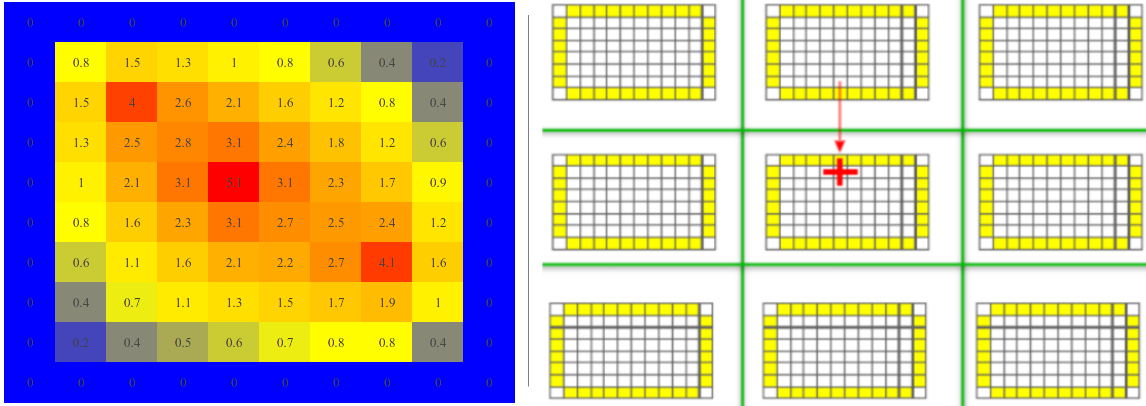
\includegraphics[width=\linewidth]{img/calomalhtran}
    \caption{Left: final temperature distribution; Right: the discretized 2D domain.}
    \label{fig:calor}
\end{figure}

Considering the chosen test problem, an initial implementation of the algorithm proposed by Balaji \cite{Balaji2017} in the C language, was easily ported to F90. The discretized 2D domain of the heat transfer problem chosen as the test problem, showing 9 subdomains divided by green lines, with their grid points and phantom zones in yellow, is shown to the right of \autoref{fig:calor}, where the red cross denotes the 5-point stencil. The left side of \autoref{fig:calor} shows the final temperature distribution over a finite surface after 500 iterations, exemplified by the grid $ 10 \times 10 $ and three arbitrarily chosen heat sources, shown as red cells, where the simulation only covers the inner grid $ 8 \times 8 $, and the initial zero temperature distribution is indicated in blue. This scheme requires splitting the original square domain into a perfect square number of square subdomains.









%%%%%%%%%%%%%%%%%%%%%%%%%%%%%%%%%%%%%%%%
\section{F90 and Python Implementations of the Test Problem}
\label{sec:implementacoes}

Several serial and parallel implementations of the test problem, described in the previous section, have been written and executed. Its description and results of processing performance are shown below. Implementations include F90, taken as a reference, standard Python, Fortran-to-Python (F2Py), Cython, and Numba (including Numba-GPU). In this work, all parallel versions of these implementations are based on the Message Passing Interface (MPI) communication library, which is wrapped by the MPI API for Python (mpi4py) \cite{Mpi4py2020}, and allows the execution of MPI processes of the Python environment. Parallelization using threads is restricted to the execution of a  Numba-compiled Python function in a GPU, which will also be discussed later. Parallelization using mpi4py allows the use of one or more computer nodes.




%----------------------------------------
\subsection{F90 Serial and Parallel}

F90 is described because it was taken as a reference for Python implementations, and was compiled with GNU gfortran. The serial version is the implementation of the algorithm described in the previous section, and the parallel version employs the standard MPI asynchronous non-blocking communication functions MPI\_ISend() and MPI\_IRecv(). At the end of each time step of the algorithm, synchronization is necessary for each sub-domain to update the phantom zones of all neighboring sub-domains. For a square grid with $ N \times N $ points and $ p $ MPI processes, each process is assigned to a sub-domain with a total of $ [(N / p) +2] \times [(N / p) +2 ] $ points. The part of the code that requires performance, updates the domain grid using the 5-point stencil (\autoref{lst:fortran}).

\begin{lstlisting}[language=Fortran, label=lst:fortran, caption={Time-consuming part of the F90 code of the test problem}]
do j = 2,by+1
  do i = 2,bx+1
    anew(i,j)= 1/2.0*(aold(i,j) + 1/4.0*(aold(i-1,j) + aold(i+1,j) + aold(i,j-1) + aold(i,j+1)))
  enddo
enddo
\end{lstlisting}




%----------------------------------------
\subsection{Standard Python Serial and Parallel}

The portability of the F90 code to Python is straightforward, without any external library except the NumPy library of numerical tools. Part of the Python loops can be executed transparently by resources from the Numpy library. The structure and sequence of the original code are preserved and executed interactively by the Python interpreter in the Jupyter Notebook environment. In this way, it is easy to modify the code or its parameters, show and record the results, perform the prototyping to check the accuracy of the algorithm and document its code and description. In this step, the user can take advantage of the modular nature of Python to selectively optimize the code, for example, by porting a specific module to F90 or replacing it with a library function for performance. Parallelization is possible using the Python multiprocessing environment which provides many ways of providing parallel execution, according to the chosen library. However, in this work, the library mpi4py (MPI for Python) was used.




%----------------------------------------
\subsection{F2Py Serial and Parallel}

F2Py is a wrapper that creates a Python module by compiling the F90 source code and requires the definition of a function with a list of arguments to be passed for the execution of the Python module, such as number of grid points, location and heat rate of sources, number of iterations, etc. In the case of the F90 code already parallelized with MPI, the module can be executed in parallel by the F90 code itself. However, if the F90 code has not yet been parallelized, the typical alternative is to use the mpi4py library (MPI for Python), but, eventually, it will be necessary to break the original code into parts and choose computationally intensive ones to parallelize with MPI. Therefore, F2Py seems more convenient when different Python modules need to be generated and called interactively. The mpi4py library resembles the F90 MPI and allows Python to perform a job using one or more shared memory computer nodes, each with multi-core processors.




%----------------------------------------
\subsection{Cython Serial and Parallel}

Cython is a static optimization compiler for the Python and Cython programming languages. It is generally used to create standard modules and to wrap C/C++ code. The Cython source code is first compiled for the C/C++ language, which is then compiled transparently by the operating system's standard compiler, generating executable machine code. Each module generated by Cython requires the definition of a corresponding standard Python function, and the performance depends on the syntactic and semantic extensions used, the resources used by the Python interpreter and the choice of libraries. The result of the compilation is a Python module that includes an API for the generated code. In the case of the serial test problem, the complete code was compiled by Cython, while in the case of the parallel code, a separate module was created compiling the double loop that updates the 2D domain, and then the mpi4py library was used. The time-consuming function that updates the domain grid using the 5-point stencil is shown in \autoref{lst:cython}.

\begin{lstlisting}[language=Python, label=lst:cython, caption={Time-consuming part of the Cython code of the test problem}]
cpdef stp(double[:,::1] anew, double[:,::1] aold,Py_ssize_t by,Py_ssize_t bx) :
  for i in range(1,bx+1) :
    for j in range(1,by+1) :
      anew[i,j] = 1/2.0*(aold[i,j] + 1/4.0*(aold[i-1,j] + aold[i+1,j] + aold[i,j-1] + aold[i,j+1]))
\end{lstlisting}




%----------------------------------------
\subsection{Numba Serial and Parallel}

Numba is a JIT (just-in-time) compiler, which compiles the code at run time and uses part of the Python language and part of the NumPy module. It uses resources from the LLVM project, which is a set of modular and reusable technologies and tools for building compilers, developed by the University of Illinois at Urbana-Campaign since 2000, which allows the generation of machine code optimized for CPU or GPU. In order to compile the code for the test problem, an approach similar to Cython was adopted, creating a Python function that embeds part of the code and is compiled by Numba. The rest of the Python code is interpreted by the standard Python, as it runs quickly. In the case of parallel code, to run on multiple cores, the mpi4py library is used, and GPU execution is also possible, as Numba supports part of the NVidia CUDA API, requiring the definition of the kernel that will run on the GPU. The processing performance for the Numba-GPU version is shown below in \autoref{ssec:gpuexec}. The time-consuming function is shown in \autoref{lst:numba}.

\begin{lstlisting}[language=Python, label=lst:numba, caption={Time-consuming part of the Numba code of the test problem}, basicstyle=\fontfamily{qhv}\fontseries{c}\selectfont\footnotesize]
@jit(nopython=True)
def kernel(anew,aold):
  anew[1:-1,1:-1] = 1/2.0*(aold[1:-1,1:-1] + 1/4.0*(aold[2:,1:-1] + aold[:-2,1:-1] + aold[1:-1,2:] + aold[1:-1,:-2]))
\end{lstlisting}








%%%%%%%%%%%%%%%%%%%%%%%%%%%%%%%%%%%%%%%%
\section{Analysis of the Parallel Performance for the Test Problem}
\label{sec:analise}


In all F90 and Python implementations of this work, the GNU 4.8.5 compiler set and the OpenMPI 4.0.1 library were employed, with the -O3 optimization flag. In the case of F90 implementations, the version compiled with the Intel 19.1.2 and Intel MPI 19.1.2 library was also tested, however the performance results were similar and, therefore, only GNU gfortran with OpenMPI is shown in the rest of this work. It is important to note that only one Bull Sequana X node was available and, therefore, in general, tests of one and several nodes were performed using Sequana B710 nodes.




%----------------------------------------
\subsection{Comments on the Performance of the CPU-executed Implementations}
\label{ssec:cpuexec}

\begin{table}
\footnotesize
\centering
\caption{Performance of test problem implementations, depending on the number of MPI processes. The best values for serial or MPI are highlighted in \red{red}. The execution time of the serial code compiled with GNU-Fortran was taken as a reference for calculating the speedup (highlighted in \blue{blue}).}
\label{tab:impl}
%\setlength{\tabcolsep}{2.6pt}
\begin{tabular}{lrrrrrrrrrr}
\toprule
&\multicolumn{9}{c}{\textbf{Processing time (s)}} \\
\cline{2-10}\vspace{-9pt} & & & & & & & & & \\
&\textbf{Serial} &\textbf{1} &\textbf{4} &\textbf{9} &\textbf{16} &\textbf{36} &\textbf{49} &\textbf{64} &\textbf{81} \\
\hline\vspace{-9pt} & & & & & & & & & \\
\textbf{F90} &\blue{19.25} &\red{21.91} &\red{7.34} &\red{6.15} &4.68 &\red{2.13} &1.89 &\red{1.23} &1.69 \\
\textbf{F2Py} &\red{18.94} &23.60 &7.45 &6.17 &\red{4.62} &2.15 &\red{1.63} &1.27 &\red{1.01} \\
\textbf{Cython} &23.97 &23.98 &7.46 &6.29 &4.69 &2.23 &1.67 &1.31 &2.06 \\
\textbf{Numba} &30.48 &30.53 &8.18 &6.33 &5.86 &3.22 &2.68 &1.79 &2.07 \\
\textbf{Python} &212.43 &227.19 &64.74 &44.78 &33.46 &15.21 &10.43 &7.85 &6.70 \\
\hline\vspace{-9pt} & & & & & & & & & \\
&\multicolumn{9}{c}{\textbf{Speedup}} \\
\hline\vspace{-9pt} & & & & & & & & & \\
\textbf{F90} &\blue{1.00} &\red{0.88} &\red{2.62} &\red{3.13} &4.11 &\red{9.04} &10.21 &\red{15.67} &11.42 \\
\textbf{F2Py} &\red{1.02} &0.82 &2.58 &3.12 &\red{4.16} &8.96 &\red{11.83} &15.14 &\red{19.03} \\
\textbf{Cython} &0.80 &0.80 &2.58 &3.06 &4.10 &8.64 &11.55 &14.74 &9.36 \\
\textbf{Numba} &0.63 &0.63 &2.35 &3.04 &3.29 &5.98 &7.19 &10.75 &9.32 \\
\textbf{Python} &0.09 &0.08 &0.30 &0.43 &0.58 &1.27 &1.85 &2.45 &2.87 \\
\hline\vspace{-9pt} & & & & & & & & & \\
&\multicolumn{9}{c}{\textbf{Parallel efficiency}} \\
\hline\vspace{-9pt} & & & & & & & & & \\
\textbf{F90} &\blue{1.00} &\red{0.88} &\red{0.66} &\red{0.35} &0.26 &\red{0.25} &0.21 &\red{0.24} &0.14 \\
\textbf{F2Py} &\red{1.02} &0.82 &0.65 &0.35 &\red{0.26} &0.25 &\red{0.24} &0.24 &\red{0.23} \\
\textbf{Cython} &0.80 &0.80 &0.65 &0.34 &0.26 &0.24 &0.24 &0.23 &0.12 \\
\textbf{Numba} &0.63 &0.63 &0.59 &0.34 &0.21 &0.17 &0.15 &0.17 &0.12 \\
\textbf{Python} &0.09 &0.08 &0.07 &0.05 &0.04 &0.04 &0.04 &0.04 &0.04 \\
\bottomrule
\end{tabular}
\end{table}

\begin{figure}[ht]
    \centering
    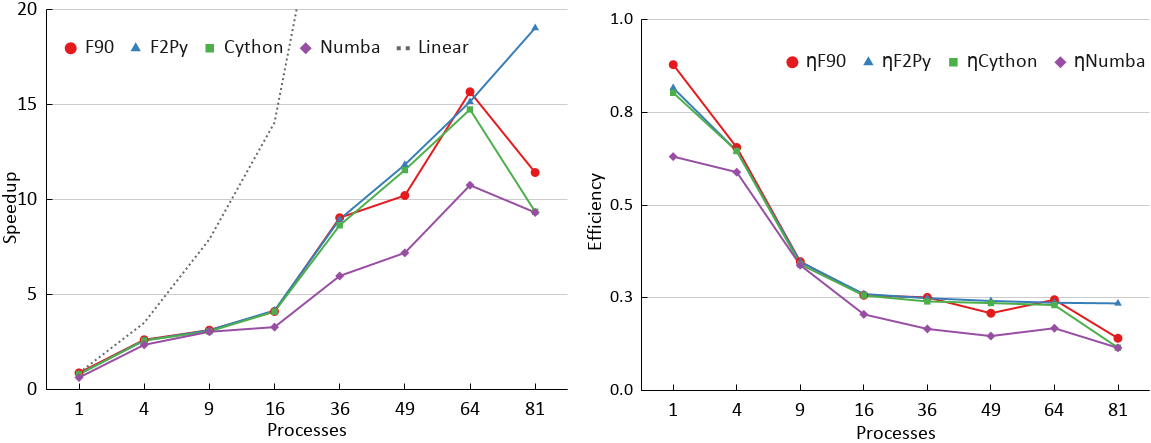
\includegraphics[clip,width=\linewidth]{img/effispee2.png}
    \caption{Speedups and efficiency of the implementations, depending on the number of processes. Dashed line denotes the linear speedup.}
    \label{fig:speedup}
\end{figure}

The \autoref{tab:impl} shows the processing times for the different implementations, in one or more Bull B710 nodes, for serial and MPI with 1, 4, 9, 16, 36, 49, 64 and 81 processes. 
These processes allow for perfect square subdomains (as explained in \autoref{sec:descricao}) in the implementation performed.
The \autoref{fig:speedup} shows the corresponding speedups calculated using the F90 serial time as a reference. In general, F90 and F2Py achieved the best performances and are followed by Cython and Numba, with Python well behind. F2Py requires few changes to the original F90 code, while Cython and Numba requires minor changes to the Python code. However, Numba's performance was comparable, from 4 to 36 processes. The low performance of Python versions shows the convenience of using implementations like F2Py, Cython, or even Numba. As can be seen, the parallel scalability is poor, since the test problem algorithm updates all points of the grid at each time step, thus requiring the exchange of boundary temperatures between neighboring subdomains, in order to update the phantom zones corresponding, requiring a lot of communication between processes, which leaves the parallel efficiency below 40\% for processes of 9 MPI or more. It can be seen that for up to 36 MPI processes, running on two Bull B710 nodes, all implementations performed similarly, except for standard Python. In the case of 81 MPI processes, which requires 4 computer nodes, the performance of the implementations has dropped significantly compared to 64 MPI processes, which requires 3 nodes. It is intended, as a future work, to investigate the reason for the performance differences between the different implementations. Besides these CPU-executed implementations, the next section briefly shows the use of a GPU-executed implementation.




\
%----------------------------------------
\subsection{Processing Performance of the Numba-GPU Implementation}
\label{ssec:gpuexec}

Numba-GPU implementation was made as an example, in order to make a very rough comparison between the performance of CPU and GPU implementations. It should not be used to draw conclusions, as such a comparison would require an extensive number of tests. This section aims to compare the performance on a single node, of: (i) implementation of a single Numba-GPU process performed on a Bull B715 node, or Bull Sequana-X node; (ii) single and serial F90 process implementations running on one or more processor cores of the Bull B715 node or Bull Sequana-X node. Note that Bull Sequana-X is a very up-to-date SDumont node, with the latest processors and GPUs. The Numba-GPU implementation was tested on a Bull B715 node using a single core, and the Tesla K40 GPU runs at 22.28~s, close to the execution time of the F90 serial implementation. The same Numba-GPU implementation performed on a Bull Sequana-X node using a single core and a single Volta V100 GPU, was performed in just 8.02~s, slightly more than most parallel implementations running with 4 MPI processes in the Bull B715 node. The implementation of the Numba-GPU required more modifications compared to the standard Python serial code than the others.
The loop was encapsulated in a function with a Numba decorator to be executed on a single GPU using just-in-time (JIT) compilation. These execution times correspond to blocks of $ 8 \times 8 $ threads in the case of the GPU V100 (node Bull Sequana-X), and blocks of $ 16 \times 16 $ threads in the case of the GPU K40 (node Bull B715). These block sizes have been optimized by trial and error. The multi-threaded single instruction (SIMT) paradigm models the execution of the GPU, with the problem domain mapped in a block grid composed of a series of threads. The blocks are then divided into warps, usually 32 threads, and executed by one of the streaming multiprocessors that make up the GPU. Numba-GPU uses a wrapper for the CUDA API in C language, providing access to most of its features. 










%%%%%%%%%%%%%%%%%%%%%%%%%%%%%%%%%%%%%%%%
\section{Final Remarks}
\label{sec:conclusao}

This work presented a comparison of the most common approaches in Python in SDumont to increase computational performance, using a given test problem. The test problem is a 2D heat transfer problem modeled by the Poisson partial differential equation, being solved by a finite difference method. Requires the calculation of a 5-point stencil over the discretized domain grid. Its serial and parallel implementations in F90 were taken as a reference to compare its performance with some serial and parallel implementations of the same algorithm available in the Python environment: F2Py, Cython, Numba, Numba-GPU and the standard Python itself. The processing times, speedups and parallel efficiencies were presented and discussed for these implementations, considering a problem size specific to the test problem.
The Python environment is a high-level interactive tool for rapid prototyping and development of computer code, allowing the integration of modules written in F90, and the use of several third-party libraries. This work intends to show that Python can also be used for HPC through APIs / libraries such as F2Py, Cython, Numba and Numba-GPU. Faster implementations are generated, porting time-consuming parts of Python code to a new function that is called from the Python program, except in the case of F2Py, which reuses an existing F90 code. The performance results of serial and parallel processing for the given test problem show that such an approach is feasible. Therefore, Python not only allows the programmer to readily develop and test the intended Python code, but also to port parts of it to obtain HPC using multiple cores and / or GPUs. The resulting code offers the portability of Python, but provides another level of modularity, since it is possible to exchange a function implemented in Cython, for example, for another one in Numba-GPU according to the available computer architecture.










%%%%%%%%%%%%%%%%%%%%%%%%%%%%%%%%%%%%%%%%
\section{Acknowledgements}

Authors thank LNCC (National Laboratory for Scientific Computing) for grant 205341 AMPEMI (call 2020-I), which allows access to the Santos Dumont supercomputer (node of the SINAPAD, the Brazilian HPC system).










%%%%%%%%%%%%%%%%%%%%%%%%%%%%%%%%%%%%%%%%
\bibliographystyle{sbc}
\bibliography{references}

\end{document}
